\documentclass[unicode,a4paper,12pt,russian]{article}
\usepackage{cmap}
\usepackage[left=1cm,right=1cm,
    top=0.5cm,bottom=0.5cm,bindingoffset=0cm]{geometry}
\usepackage[dvips]{graphicx}
\usepackage[unicode=true]{hyperref}
\usepackage[cm-default]{fontspec}
\usepackage{xunicode}
\usepackage{xltxtra}
\usepackage{polyglossia}
\usepackage{wrapfig}
\usepackage{color}
\usepackage{xcolor,mdframed}
\usepackage{subfigure}
\usepackage{textcomp}
\usepackage{listings}
\definecolor{dkgreen}{rgb}{0,0.6,0}
\definecolor{mauve}{rgb}{0.58,0,0.82} 
\newenvironment{important}[1][]{%
   \begin{mdframed}[%
      skipabove=0.7\baselineskip, skipbelow=0.7\baselineskip,
      splitbottomskip=2pt, splittopskip=4pt, #1]%
   \makebox[0pt]{% ignore the withd of !
      \smash{% ignor the height of !
         \fontsize{32pt}{32pt}\selectfont% make the ! bigger
         \hspace*{-19pt}% move ! to the left
         \raisebox{-2pt}{% move ! up a little
            {\color{red!70!black}\sffamily\bfseries !}% type the bold red !
         }%
      }%
   }%
}{\end{mdframed}}
\lstset{ %
  language=bash,
  backgroundcolor=\color{white},
  frame=single,
  rulecolor=\color{black},
  tabsize=2,
  breaklines=true,
  breakatwhitespace=true, 
  keywordstyle=\color{blue},
  commentstyle=\color{dkgreen},
  stringstyle=\color{mauve} 
}
\defaultfontfeatures{Mapping=tex-text}
\setmainfont{Liberation Serif}
\newfontfamily\cyrillicfont{Liberation Serif}
\setmonofont{Liberation Mono}
\newfontfamily\cyrillicfonttt{Liberation Mono}
\setsansfont{Liberation Sans}
\newfontfamily\cyrillicfont{Liberation Sans}
\setdefaultlanguage[spelling=modern]{russian}
\setotherlanguage{english}
\graphicspath{{../images/}}
\begin{document}

\begin{center}
\LARGE \textbf{Обходим Великий Российский Файрвол}\\
\large Часть 1 из 5\\
\normalsize\textbf{В России официально установлена цензура Интернета. Но контролировать Интернет не так просто, как это может показаться с первого взгляда.}
\end{center}
\begin{figure}[h]
\center{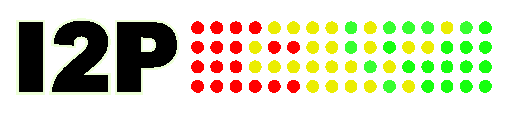
\includegraphics[width=0.25\linewidth]{I2P}}
\end{figure}
\textbf{I2P} --- анонимная оверлейная сеть, использующая принцип чесночной маршрутизации, исходные коды которой распространяются на условиях нескольких свободных лицензий. В отличии от Tor, который в первую очередь направлен на доступ к сайтам обычного интернета (хотя в нем и существуют скрытые сервисы, аналогичные ипсайтам в I2P, а в I2P можно получить доступ к внешнему Интернету, используя аутпрокси), основной целью I2P является доступ именно к скрытым ресурсам --- ипсайтам. Ипсайт от обычного вебсайта отличает только его нахождение в сети I2P.
\begin{important}
Никогда не используйте анонимные сети с настройками, которые позволяют использовать Интернет в одном браузере в обход самой сети. В этом случае будет достаточно вставить любое изображение из внешнего Интернета, чтобы получить ваш реальный IP-адрес.
\end{important}
\subsection*{Установка}
Для установки посетите \url{http://i2p2.de} или установите пакет с помощью пакетного менеджера вашего дистрибутива.
\subsection*{Использование}
\begin{important}
Не используйте аутпрокси для передачи конфиденциальных данных, владелец аутпрокси видит трафик нешифрованным.
\end{important}
После установки настройте свой браузер на использование HTTP-прокси 127.0.0.1:4444 и посетите страницу \url{http://127.0.0.1:7657}. Перед вами консоль маршрутизатора I2P --- место, из которого можно управлять всеми настройками I2P.\\
Для начала перейдите в меню <<Настройки I2P>> (\url{http://127.0.0.1:7657/config}) и установите ограничения скорости в соответствии со скоростью вашего интернета.\\
Остальные настройки можно оставить по умолчанию. Подождите некоторое время для полноценной интеграции с сетью, после чего вы сможете полноценно пользоваться сетью. Роутер желательно не выключать, так как при его перезапуске потребуется придется повторить этот процесс.\\
В I2P отсутствуют корневые DNS-сервера, копия адресной книги хранится на каждом роутере. На \url{http://rus.i2p} вы можете найти дополнительный список подписок, который можно добавить в susidns.
\subsection*{Некоторые ипсайты}
\begin{enumerate}
\item \url{http://forum.i2p} --- главный форум, есть рускоязычный раздел.
\item \url{http://rus.i2p} --- русская I2P-вики.
\item \url{http://pastethis.i2p} --- pastebin-подобный ресурс.
\item \url{http://flibusta.i2p} --- зеркало Флибусты, крупной библиотеки электронных книг.
\item \url{http://tracker.rus.i2p} --- русский торрент-трекер в I2P.
\end{enumerate}
\vfill
\scriptsize Создано на основе материалов из <<Настольной книги анонима>> --- \url{anonhandbook.org}, \url{anonhandbook.i2p}, \url{oxgzwiiypou6udlp.onion}
\normalsize

\begin{center}
\LARGE \textbf{Обходим Великий Российский Файрвол}\\
\large Часть 2 из 5\\
\normalsize\textbf{В России официально установлена цензура Интернета. Но контролировать Интернет не так просто, как это может показаться с первого взгляда.}
\end{center}
\begin{figure}[h]
\center{
\includegraphics[width=0.25\linewidth]{Tor}}
\end{figure}
\textbf{Tor} --- анонимная оверлейная сеть, использующая принцип луковой маршрутизации, исходные коды которой распространяются на условиях лицензии BSD.\\
\textbf{Луковая маршрутизация} --- технология анонимного обмена информацией, использующая многократное шифрование и пересылку через цепочки узлов. Каждый луковый маршрутизатор в цепочке удаляет слой шифрования и пересылает сообщение дальше, согласно полученным инструкциям, где все повторится. И так до тех пор, пока сообщение не достигнет адресата. Такое название технология получила из-за сходства данного процесса с очисткой луковицы.
\begin{important}
Никогда не используйте анонимные сети с настройками, которые позволяют использовать Интернет в одном браузере в обход самой сети. В этом случае будет достаточно вставить любое изображение из внешнего Интернета, чтобы получить ваш реальный IP-адрес.
\end{important}
\subsection*{Установка}
Для установки посетите \url{https://torproject.org} или установите пакет с помощью пакетного менеджера вашего дистрибутива.
\subsection*{Использование}
\begin{important}
Не забывайте, что при использовании обычного Интернета через Tor, последняя нода в цепочке (exit-нода) видит трафик нешифрованным.
\end{important}
Самым простым способом использования Tor является установка Tor Browser Bundle. Просто скачайте его с \url{https://torproject.org/projects/torbrowser.html}, распакуйте и запустите.\\
Вы также можете установить Tor и задать в настройках приложений, которые вы хотите через него использовать, адрес socks5-прокси 127.0.0.1:9050.\\
Для использования приложений через Tor, не имеющих настроек прокси, скачайте torsocks --- \url{https://code.google.com/p/torsocks}.
\subsection*{Некоторые скрытые сервисы}
\begin{enumerate}
\item \url{http://dppmfxaacucguzpc.onion} --- TorDir, каталог скрытых сервисов.
\item \url{http://jhiwjjlqpyawmpjx.onion} --- TorMail, электронная почта в Tor.
\item \url{http://silkroadvb5piz3r.onion} --- Silk Road, анонимная торговая площадка, принимающая оплату в Bitcoin.
\item \url{http://4eiruntyxxbgfv7o.onion/pm} --- TorPM, сервис обмена сообщениями.
\item \url{http://c4wcxidkfhvmzhw6.onion} --- PrivacyBox, сервис анонимных контактных форм.
\end{enumerate}
\vfill
\scriptsize Создано на основе материалов из <<Настольной книги анонима>> --- \url{anonhandbook.org}, \url{anonhandbook.i2p}, \url{oxgzwiiypou6udlp.onion}
\normalsize

\begin{center}
\LARGE \textbf{Обходим Великий Российский Файрвол}\\
\large Часть 3 из 5\\
\normalsize\textbf{В России официально установлена цензура Интернета. Но контролировать Интернет не так просто, как это может показаться с первого взгляда.}
\end{center}
\textbf{VPN} --- технология, позволяющая создавать сети поверх существующего Интернет-подключения. Из-за высокой скорости работы, простоты настройки и шифрования трафика от клиента до VPN-провайдера часто используется как средство сокрытия реального IP-адреса при доступе в Интернет. VPN-провайдеры обычно предоставляют свои услуги на платной основе.\\
\textbf{SSH} --- протокол, созданный для безопасной передачи данных. Часто используется для удаленного управления другими компьютерами, но может использоваться и для создания туннелей.\\
\textbf{SSH-туннель} --- туннель, созданный с помощью SSH-соединения и используемый для передачи данных. Существуют организации, предоставляющие SSH-туннелирование на платной основе.
\subsection*{Использование}
\begin{important}
Не забывайте, что хозяин VPN-сервиса или SSH-туннеля видит трафик нешифрованным.
\end{important}
При использовании VPN, следуйте инструкциям, полученным от вашего VPN-провайдера.\\
SSH-туннели настраиваются так:
\begin{lstlisting}
ssh -D localhost:port login@address
\end{lstlisting}
port --- порт, трафик на который будет пропускаться через SSH-туннель.\\
login --- ваш логин на удаленном сервере.\\
address --- адрес удаленного сервера.\\
После этого установите в приложениях, трафик которых вы хотите туннелировать, например, в браузере, адрес SOCKS-прокси localhost с портом, который вы указали в предыдущем шаге.
\subsection*{Некоторые VPN-провайдеры}
\begin{enumerate}
\item \url{https://ipredator.se}
\item \url{https://kebrum.com}
\item \url{https://relakks.com}
\item \url{https://vpntunnel.se}
\item \url{http://ivacy.com}
\end{enumerate}
\subsection*{Некоторые провайдеры SSH-туннелей}
\begin{enumerate}
\item \url{https://tunnelr.com}
\item \url{http://torvpn.com}
\item \url{http://vpnsecure.me}
\item \url{http://guardster.com}
\item \url{http://anonyproz.com}
\end{enumerate}
\vfill
\scriptsize Создано на основе материалов из <<Настольной книги анонима>> --- \url{anonhandbook.org}, \url{anonhandbook.i2p}, \url{oxgzwiiypou6udlp.onion}
\normalsize

\begin{center}
\LARGE \textbf{Обходим Великий Российский Файрвол}\\
\large Часть 4 из 5\\
\normalsize\textbf{В России официально установлена цензура Интернета. Но контролировать Интернет не так просто, как это может показаться с первого взгляда.}
\end{center}
\textbf{JonDo} (\textbf{JonDonym}, также \textbf{Java Anon Proxy} или \textbf{JAP}) --- программное обеспечение, представляющее доступ к цепочке прокси-серверов.
\subsection*{Установка}
Для установки посетите \url{https://anonymous-proxy-servers.net} или установите пакет с помощью пакетного менеджера вашего дистрибутива.
\subsection*{Использование}
\begin{important}
Не забывайте, что хозяева выходных нод видят трафик нешифрованным.
\end{important}
JonDo напоминает Tor, но в отличии от Tor, где каждый доброволец может поднять как промежуточный сервер, так и exit-ноду, JonDo опирается на помощь отдельных организаций. Однако, Tor может использоваться в цепочке JonDo, для этого достаточно добавить адрес socks5-прокси Tor.\\
Бесплатная версия позволяет проксировать только HTTP и HTTPS трафик, в платной версии доступно все, а также нелимитирована скорость.\\
Для использования запустите JonDo и настройте браузер на использование прокси-сервера\\127.0.0.1:4001.
\subsection*{Недостатки}
\begin{enumerate}
\item В бесплатной версии можно проксировать только HTTP и HTTPS.
\item В бесплатной версии скорость ограничена до 30--50 кБит/с.
\item В бесплатной версии размер передаваемого файла ограничен 2 МБ.
\item Число нод очень сильно ограничено.
\end{enumerate}

\vfill
\scriptsize Создано на основе материалов из <<Настольной книги анонима>> --- \url{anonhandbook.org}, \url{anonhandbook.i2p}, \url{oxgzwiiypou6udlp.onion}
\normalsize

\begin{center}
\LARGE \textbf{Обходим Великий Российский Файрвол}\\
\large Часть 5 из 5\\
\normalsize\textbf{В России официально установлена цензура Интернета. Но контролировать Интернет не так просто, как это может показаться с первого взгляда.}
\end{center}
\textbf{Прокси-сервер} --- сервер, который позволяет пропускать через себя пользовательский трафик.\\
\textbf{Веб-прокси} --- веб-страница, которая позволяет пользователю получить контент с заданного адреса через себя.
\subsection*{Использование}
\begin{important}
Не забывайте, что хозяева прокси-серверов и анонимайзеров видят трафик нешифрованным.
\end{important}
\begin{important}
Некоторые прокси-сервера передают заголовок X-Forwarded-For с реальным IP-адресом клиента.
\end{important}
В случае использования прокси, просто задайте его адрес в настройках браузера и других приложений, которые вы хотите использовать через прокси.\\
В случае использования веб-прокси, перейдите на его страницу и введите адрес сайта, который вы хотете посетить.
\subsection*{Списки открытых прокси}
\begin{enumerate}
\item \url{http://xroxy.com}
\item \url{https://hidemyass.com/proxy-list}
\item \url{http://freeproxy.ch}
\item \url{http://proxylists.net}
\item \url{http://nntime.com}
\end{enumerate}
\subsection*{Некоторые веб-прокси}
\begin{enumerate}
\item \url{https://hidemyass.com}
\item \url{http://anonymouse.org}
\item \url{http://hide.pl}
\item \url{http://hideme.ru}
\item \url{http://guardster.com/free/}
\end{enumerate}

\vfill
\scriptsize Создано на основе материалов из <<Настольной книги анонима>> --- \url{anonhandbook.org}, \url{anonhandbook.i2p}, \url{oxgzwiiypou6udlp.onion}
\normalsize


\end{document}
